\chapter{Introduction}
\label{ch:intro}

% Typically 4-7 pages.

% ------------------------------------------------------------
\section{Background} % (fold)
\label{sec:Problem}

% Introduce the domain of information extraction.
% Motivation – a real issue?, What is the research context? What is the state-of-art?

The World Wide Web contains a vast amount of information, counting in billions of web pages \cite{signorini2005a}. Mostly it is unstructured or semi-structured documents, making it difficult to process the data directly by machines. As a result, sharing and reusing knowledge across multiple parties is hardly possible without human interaction.

Addressing the need to automatically extract and process large volumes of accessible information, machine needs to extract loosely-structured data from web sources and populate databases with well-structured data for further handling. The problem can be seen as information extraction problem for web pages. 

There are many use cases for sharing data between web-based applications with no dedicated integration capabilities. Some examples include extracting product price information from competitor on-line shops, or integrating with an online scheduling application which has no application programming interface (API). In both cases data is presented to the user via the web browser and no special care was taken to make it easy for automatic extraction.


% ------------------------------------------------------------
\section{The Problem}

% Since you have a goal, there must be some problem that you are trying to solve. Explain this problem. What people in the real world are affected by the problem that concerns you? It is best if your grandmother understands this section.
% What is broken/missing (the ”gab”), Thesis or Problem statement 
 
% Web wrapping
Most of the pages on the web are HTML documents. Many websites use view templates to generate individual pages on the server side. Thus, a list of objects on a page, generated by a template, has a repeating structural pattern. HTML has a tree structure and can be viewed as a labeled ordered rooted tree. To extract information from the webpage, one needs to query a node in a tree. The program that performs the actual information extraction (IE) task from webpages is called a \emph{web wrapper}. The web wrapper query can be expressed in a number of standartized notations, e.g. XPath, CSS selectors, etc.

% Robustness
For a webpage, writing a query that extracts a certain piece of information is a straight forward task. A query can be written in many ways and still uniquelly target the same node in HTML tree. The problem gets really interesting when one takes into consideration that websites are maintained and evolve over time. A slight change of the HTML document structure might result in a non-functional wrapper.

% Data records
In this paper, we focus on web pages that contain a list of similar items, e.g. a list of products. These \emph{data records} are displayed in a web page with regular structural pattern. Figure~\ref{fig:amazon-books-html} provides an example, a part of the web page that lists four books. The full description of each book is a data record. The actual HTML tag tree for the page in Figure~\ref{fig:amazon-books-html} is given in Figure~\ref{fig:amazon-books-tree}.

\begin{figure}[h]
	\centering
	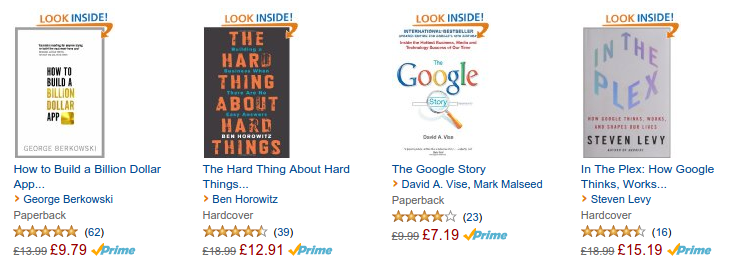
\includegraphics[width=1.0\textwidth]{figures/amazon-books}
	\caption{An example of four data records.}
	\label{fig:amazon-books-html}
\end{figure}

\begin{figure}[h]
	\centering
	\Tree [.table 
			[.tr 
				[.td [.img ] ]
				[.td [.img ] ]
				[.td [.img ] ]
				[.td [.img ] ]
			]
			[.tr 
				[.td 
					[.a
						[.\textit{How to Build...} ]
					]
					[.a
						[.\textit{George...} ]
					]
					[.span 
						[.\textit{Hardcover} ]
					]
					[. ... ]
				]
				[. ... ]
			]
		]
	\caption{Tag tree of the page in Figure~\ref{fig:amazon-books-html}}
	\label{fig:amazon-books-tree}
\end{figure}

\begin{figure}[h]
	\centering
    \begin{tabularx}{\textwidth}{ | l | l | }
		\hline
		\textbf{Title} & \textbf{Author} \\ 
		\hline
		How to Build a Billion Dollar App ... & George Berkowski \\ 
		\hline
		The Hard Thing About Hard Things ... & Ben Horowitz \\ 
		\hline
		The Google Story & David A. Vise, Mark Malseed \\ 
		\hline
		In The Plex: How Google Thinks, Works ... & Steven Levy \\ 
		\hline
    \end{tabularx}
\end{figure}

% Annotation and automation
A \emph{record-level wrapper} extracts multiple records from a single web page, while a \emph{page-level wrapper} extracts a single piece of information from a page. Wrappers rely on extraction rules to identify the data field to be extracted. Most wrapper generation techniques learn the extraction rules from a training set. A user manually \emph{annotates} sample pages by pointing to tree nodes with relevant pieces of information.

% Subject of this paper
Building a robust and fast record-level wrapper from a single annotated web page within reasonable execution time is the subject of this paper. Defining wrapper \emph{robustness} is a problem of its own. Some format definitions will be shown later. Informally, it's the wrapper that has the lowest odds of breaking after any changes to the web page structure.

% Relevance
The problem of building a robust wrapper is relevant in many areas, inluding web application integration, web user interface test automation, and web scrapping.


% ------------------------------------------------------------
\section{Objectives}

% After the motivation (why) explain in detail what the goal is. If your project contains an element of research (which is good) the goal is more like a hypothesis. In other words, your goal is to investigate some particular method to verify its usefulness for some particular purpose (verify the hypothesis).
The goal of this thesis is to design and test an algorithm for fast and robust record-level wrapping of (future) web pages, having only a single annotated HTML \emph{snapshot}, i.e. a specific document version at a given time. Futhermore, the algorithm is constrained with the following limitations and assumptions:

\begin{enumerate}
	\item There is a single annotated snapshot of a web page, i.e. training set of one.
	\item The wrapper must be robust and correctly extract information from the future web page versions.
	\item The wrapper must be reasonably fast on commodity hardware.
\end{enumerate}

% TODO I suggest that you take a little concrete example and explain your method in terms of that, so that the reader can see the input HTML tree, what you use each of the three methods for, and what you get as result.

The Figure~\ref{fig:record-level-wrapping} illustrates and example of annotated initial snapshot of the document. The user marks the position of data attribute at any record (see left-hand side). Subsequently, a new snapshot of the same but page is given. The location of picture and description in each record has changed. The algorithm locates six data records in the new page and exact positions of the same data attribute in each record (see right-hand side).

\begin{figure}[h]
	\centering
	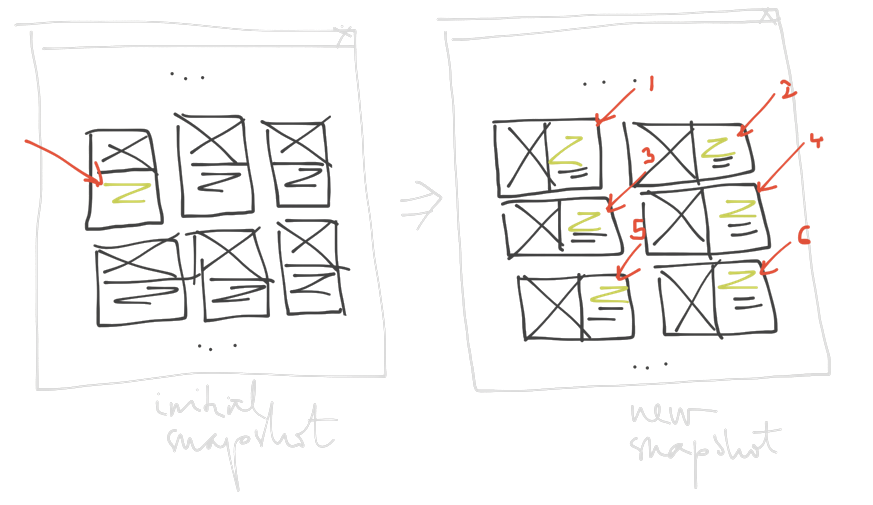
\includegraphics[width=1\linewidth]{figures/record-level-wrapping}
	\caption{Record-level wrapping example.}
	\label{fig:record-level-wrapping}
\end{figure}


% ------------------------------------------------------------
\section{Contribution}
\label{sec:contribution}

% What methods are used?
% Briefly references to related research (just the main references – more references in chapter ”Related research” or throughout the thesis)
% Emphasize your own contribution: what is original or new?

% 2. What can other methods do?
Current approaches suffer from a number of problems. First, many wrapping techniques lack formal definition of robustness and are based on a number of heuristics [TODO refs]. Other techniques require large training sets[TODO refs]. Most of the methods are based on enumeration and are slow [TODO refs]. Finally, some wrappers assume single data record per page. While there are solutions addressing individual steps, there is no coherent framework for fast and robust future record-level wrapping given single annotated snapshot of an HTML document.

% 1. Why did you choose to combine these three methods? Are there alternatives?
In this paper, we present a new method for fast and robust record-level data extraction. The method builds on three lines of work and combines them in a novel way: \emph{data region mining} \cite{liu2009a} to recognize template generated areas on a web page, \emph{probabilistic wrapper induction} \cite{DBLP:journals/pvldb/ParameswaranDGR11} to extract data from a single data record in a robust way, and \emph{partial tree alignment} \cite{zhai2005a} to repeatedly extract data from multiple records. 

% 3. Why do you think that your method will be better? (This is in fact the thesis of your thesis.) You should elaborate a bit on each of these points. That is, relate your approach to the state-of-the-art and argue for your choice.
Data records on the web and probabilistic change models for trees have not been combined before into a coherent system. We demonstrate that our method is both fast and accurate. (TODO more about the experiment setup and findings later) We also show that chosen techniques can be optimized / fine-tuned for specific use-case to get better performance and accuracy.

% TODO
We have implemented the method in Java and used the implementation to evaluate and fine tune the method. The evaluation shows that ... achieves higher accuracy, precision and robustness than the alternatives approaches...

% TODO
The contribution can be summed up:

\begin{enumerate}
	\item A novel algorithm for robust record-level wrapping using single annotated page as a training set.
	\item A full implementation in Java, parametrized ... (available at \url{https://bitbucket.org/mantiniss/thesis-wrapper}).
	\item An experimental evaluation and comparison of different algorithm variations based on about XXX HTML pages taken from YY web sites over a period of more than a ZZZ.
\end{enumerate}

% TODO Why? Alternatives? 



% What I managed to do, though, is to narrow down my focus to the tool-for-the-job – a tree edit-distance application. There are three recent papers that build on this idea \cite{DBLP:conf/sigmod/DalviBS09}, \cite{DBLP:journals/pvldb/ParameswaranDGR11}, \cite{DBLP:conf/wism/LiuWYL12}.

% While the idea of robust wrappering is not new, the core difference from earlier systems is the unique combination of ideas and tools that are optimized for performance.

% Here the idea of computing edit-distance between two trees (or DOMs) is introduced, robustness is defined formally, and later dynamic algorithm for finding the optimal wrapper is designed. My contribution was to implement the algorithm, optimize the performance using the latest research, and improve the algorithm to support multiple result sets (as opposed to single node from the query).

% I would carry out an empirical research and experiment with variations: (1) precompute various minimum cost models, (2) try $O(n)$ heuristics for calculating min diff between two trees vs $O(n^3)$ traditional approach, (3) try different candidate wrapper generation techniques.

% Build on the basis of \cite{DBLP:journals/pvldb/ParameswaranDGR11}, implement optimizations and run empirical experiments: (1) think of change probabilities model, (2) optimize for multiple extractions, (3) parallize with functional implementation, (4) analyze for multiple distinguished nodes extraction, (5) identify repeating elements of page + the base and run wrapper in each subtree of the base.

% We could compare various XPath enumeration techniques, eg Dalvi'09, vs Probabilistic model Parameswaran'11.

% Add visual features and content patterns to the structural model \cite{Chidlovskii:2006:DES:1142473.1142555}. (Visual features, which are obtained from web browsers API, enhance understanding of semantic similarity between web page elements.) Improve Parameswaran'11 with content models (see wrapper repairs).

% For multiple nodes per wrapper on same page, recognize data regions first Zhai and run all the wrapper inducers later. Utilize record-level wrapper induction \cite{DBLP:conf/cikm/ZhengSWG09}.

% According to (Myllymaki \& Jackson, 2002), robustness can be achieved by “relying less on page structure and more on content.” Use more of that. We think that in addition to this, the total number of hops should be minimized because every additional hop increases the risk of failure.

% Dalvi'09 on change model learning:
% - same set of tags appear in the top list for insertions and deletions, i.e. a, br tend to be be more volatile.
% - same sets of tags appear in the top of the list. most volatile tags may not depend heavilyt on the data?
% - yet tr,td are more prominent in some websites. also ul, li. depends on how layouts are made.


% ------------------------------------------------------------
\section{Organization}

We define the main concepts of the problem domain in Chapter 2. In Chapter 3 we discuss current state of the art across relevant lines of research. Chapters 4-8 describe our method in detail and elaborate on the design decisions. We present the empirical experiment results in Chapter 9. The thesis is conluded with findings discussion and future research direction.


% vim:wrap linebreak nolist:
